\clearpage		\large
\chapter{Test Fixture Drawings} \label{App:test_figure_drawings}

\begin{table}[H]
\centering
\begin{tabular}{|L{0.23\textwidth}|C{0.08\textwidth}|C{0.08\textwidth}|C{0.08\textwidth}|C{0.08\textwidth}|L{0.25\textwidth}|}
\hline
Item 								&Length (in) 	&Width (in) 	&Height (in) 	&Weight (lbs.) 	&Material \\ \hline \hline
King Mattress 						&79 			&71 			&10 			&76 			&52\% Polyurethane Foam, 30\%, Blended Cotton Batting, \& 18\% Polyester Fiber Batting \\ \hline
King Box Spring 					&78 			&35 			&7 				&46 			&59\% Fiber Pad, 41\% Blended Cotton Batting \& Wood Frame \\ \hline
King Headboard 						&78 			&24 			&1 				&54 			&Medium Density Fiberboard \\ \hline
Pillow 								&23.5 			&17 			&4 				&1.5 			&Filling - All Polyester, Cover - 100\% Cotton \\ \hline
Comforter 							&104 			&92 			&1 				&4.6 			&Cover - 100\% Polyester, Fill - 100\% Polyester \\ \hline
Mattress Topper 4 in 				&78 			&75 			&3.875 			&16  			&Viscoelastic Polyurethane Foam Pad 100\% \\ \hline
Night Stand 						&18 			&27 			&23.375 		&60 			&Solid Wood \\ \hline
Dresser 							&22.125 		&36 			&34.25 			&120 			&Wood \& Plywood \\ \hline
Curtain (Small) 					&39 			&73 			&0.125 			&4.5 			&Flame Retardant \& Synthetic Fibers \\ \hline
Sofa Chair (Yellow/Green) 			&31.25 			&31 			&39 			&54 			&Polyester Fiber 75\%, Polyurethane Foam 25\%, Pillow - Polyurethane Foam 90\%, Polyester Batting 10\% \\ \hline
Sofa Chair (Red Lines) 				&34.5 			&34 			&32 			&63 			&Urethane Foam 100\% \\ \hline
Sofa Chair (Red Swirl) 				&34 			&34 			&32 			&70 			&Blended Cotton Felt 100\%, Cushion, Polyurethane Foam 100\% \\ \hline
Sofa Chair (Red Diamond) 			&35 			&35 			&34 			&69 			&Polyurethane Foam (Blended Cotton or, Polyester when used is less than 10\%) \\ \hline
\end{tabular}
\caption{Bedroom Fuel Load Information}
\label{table:bd_fuel_weights}
\end{table}

\begin{table}[H]
\centering
\begin{tabular}{|L{0.23\textwidth}|C{0.08\textwidth}|C{0.08\textwidth}|C{0.08\textwidth}|C{0.08\textwidth}|L{0.25\textwidth}|}
\hline
Item 								&Length (in) 	&Width (in) 	&Height (in) 	&Weight (lbs.) 	&Material \\ \hline \hline
Curtain (Large) 					&107 			&73 			&0.125 			&13.7 			&Flame Retardant \& Synthetic Fibers \\ \hline
Mattress Topper 5 in 				&77.5 			&76.25 			&4.625 			&20.1  			&Urethane Foam \\ \hline
Kitchen Table 						&52 			&26 			&24.5 			&29.1 			&Particleboard \& Wood \\ \hline
Straight Chair (Pink) 				&18 			&19 			&33 			&15.2 			&Wood \& Upholstery \\ \hline
Straight Chair (Blue) 				&19 			&19 			&38.875 		&14.9 			&Wood \& Upholstery \\ \hline
Bookcase 							&11.5 			&24.625 		&71.25 			&46 			&Particleboard \\ \hline
TV Stand 							&22.125 		&36 			&34.25 			&120 			&Wood \& Plywood \\ \hline
Sofa 								&35 			&77 			&30.5 			&255 			&Polyurethane Foam 50\%, Polyester Fiber 50\%,\& Wood Frame \\ \hline
Sofa Chair (Striped) 				&33 			&35 			&33.5 			&65 			&Polyurethane Foam 75\% Polyester Fiber 25\% \\ \hline
Ottoman 							&19.75 			&25.5 			&16 			&21.3 			&Upholstery \\ \hline
Coffee Table 			 			&30 			&18 			&18.25 			&24.4 			&Particleboard \& Wood \\ \hline
End Table 			 				&24.25 			&24.25 			&22.125 		&32.1 			&Solid Wood \\ \hline
Table Lamp Base 					&5.75 			&5.25 			&31.25 			&5.9 			&Glass, Metal  \\ \hline
Table Lame Shade 					&14.375 		&14.375 		&  				&  				&Cloth Shade \\ \hline 
\end{tabular}
\caption{Kitchen and Living Room Fuel Load Information}
\label{table:k_lv_fuel_weights}
\end{table}

\begin{table}[H]
\centering
\begin{tabular}{|L{0.23\textwidth}|C{0.08\textwidth}|C{0.08\textwidth}|C{0.08\textwidth}|C{0.08\textwidth}|L{0.25\textwidth}|}
\hline
Item 								&Length (in) 	&Width (in) 	&Height (in) 	&Weight (lbs.) 	&Material \\ \hline \hline
Bedroom 1 Carpet (Room) 			&13.33			&12.75			&				&47.6			& \\ \hline
Bedroom 1 Carpet (Closet)			&7.5			&2.9			&				&6				& \\ \hline
Bedroom 1 Carpet Padding (Room)		&13.33			&12.75			&				&27.2			& \\ \hline
Bedroom 1 Carpet Padding (Closet)	&7.5			&2.9			&				&3.4			& \\ \hline	 	 
Bedroom 2 Carpet (Room) 			&11				&12.75			&				&39.3			& \\ \hline
Bedroom 2 Carpet (Closet)			&6.1			&1.9			&				&3.2			& \\ \hline
Bedroom 2 Carpet Padding (Room)		&11				&12.75			&				&22.4			& \\ \hline
Bedroom 2 Carpet Padding (Closet)	&6.1			&1.9			&				&1.8			& \\ \hline	  
Bedroom 3 Carpet 					&11				&12.75			&				&39.3			& \\ \hline
Bedroom 3 Carpet Padding 			&11				&12.75			&				&22.4			& \\ \hline	 
Bedroom 4 Carpet 					&11.1			&12.75			&				&39.6			& \\ \hline
Bedroom 4 Carpet Padding 			&11.1			&12.75			&				&22.6			& \\ \hline	 
Kitchen Carpet 						&12.75			&18.8			&				&67.1			& \\ \hline
Kitchen Carpet Padding 				&12.75			&18.8			&				&38.3			& \\ \hline	 
Living Room Carpet					&16.1			&19.1			&				&85.5			& \\ \hline
Living Room Carpet Padding 			&16.1			&19.1			&				&49.5			& \\ \hline	
\end{tabular}
\caption{Carpet and Padding Fuel Load Information}
\label{table:carpet_padding_fuel_weights}
\end{table}

\begin{sidewaysfigure}
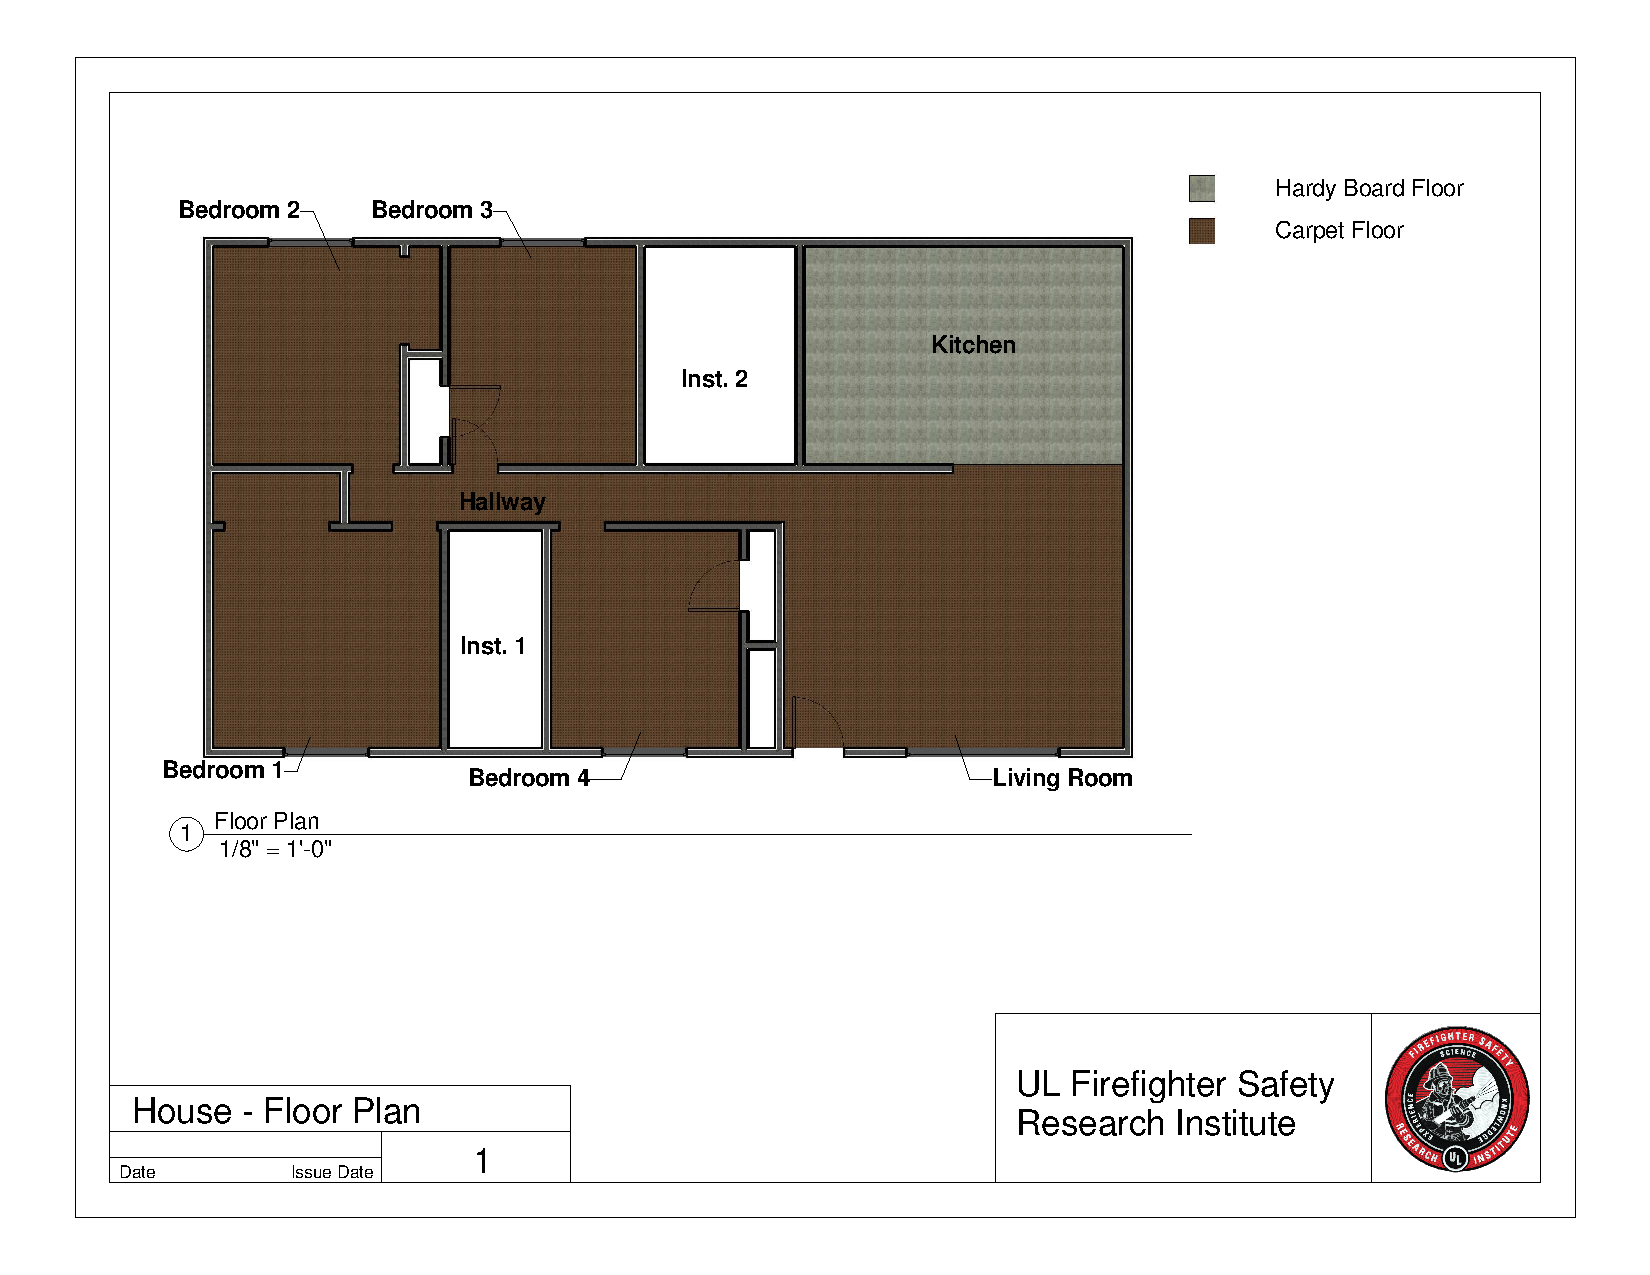
\includegraphics[width=\textheight]{../0_Images/Appendix_Figures/Floor_Plan}
\caption[]{Test Fixture Floor Plan}
\label{fig:appendix_floorplan}
\end{sidewaysfigure}

\begin{sidewaysfigure}
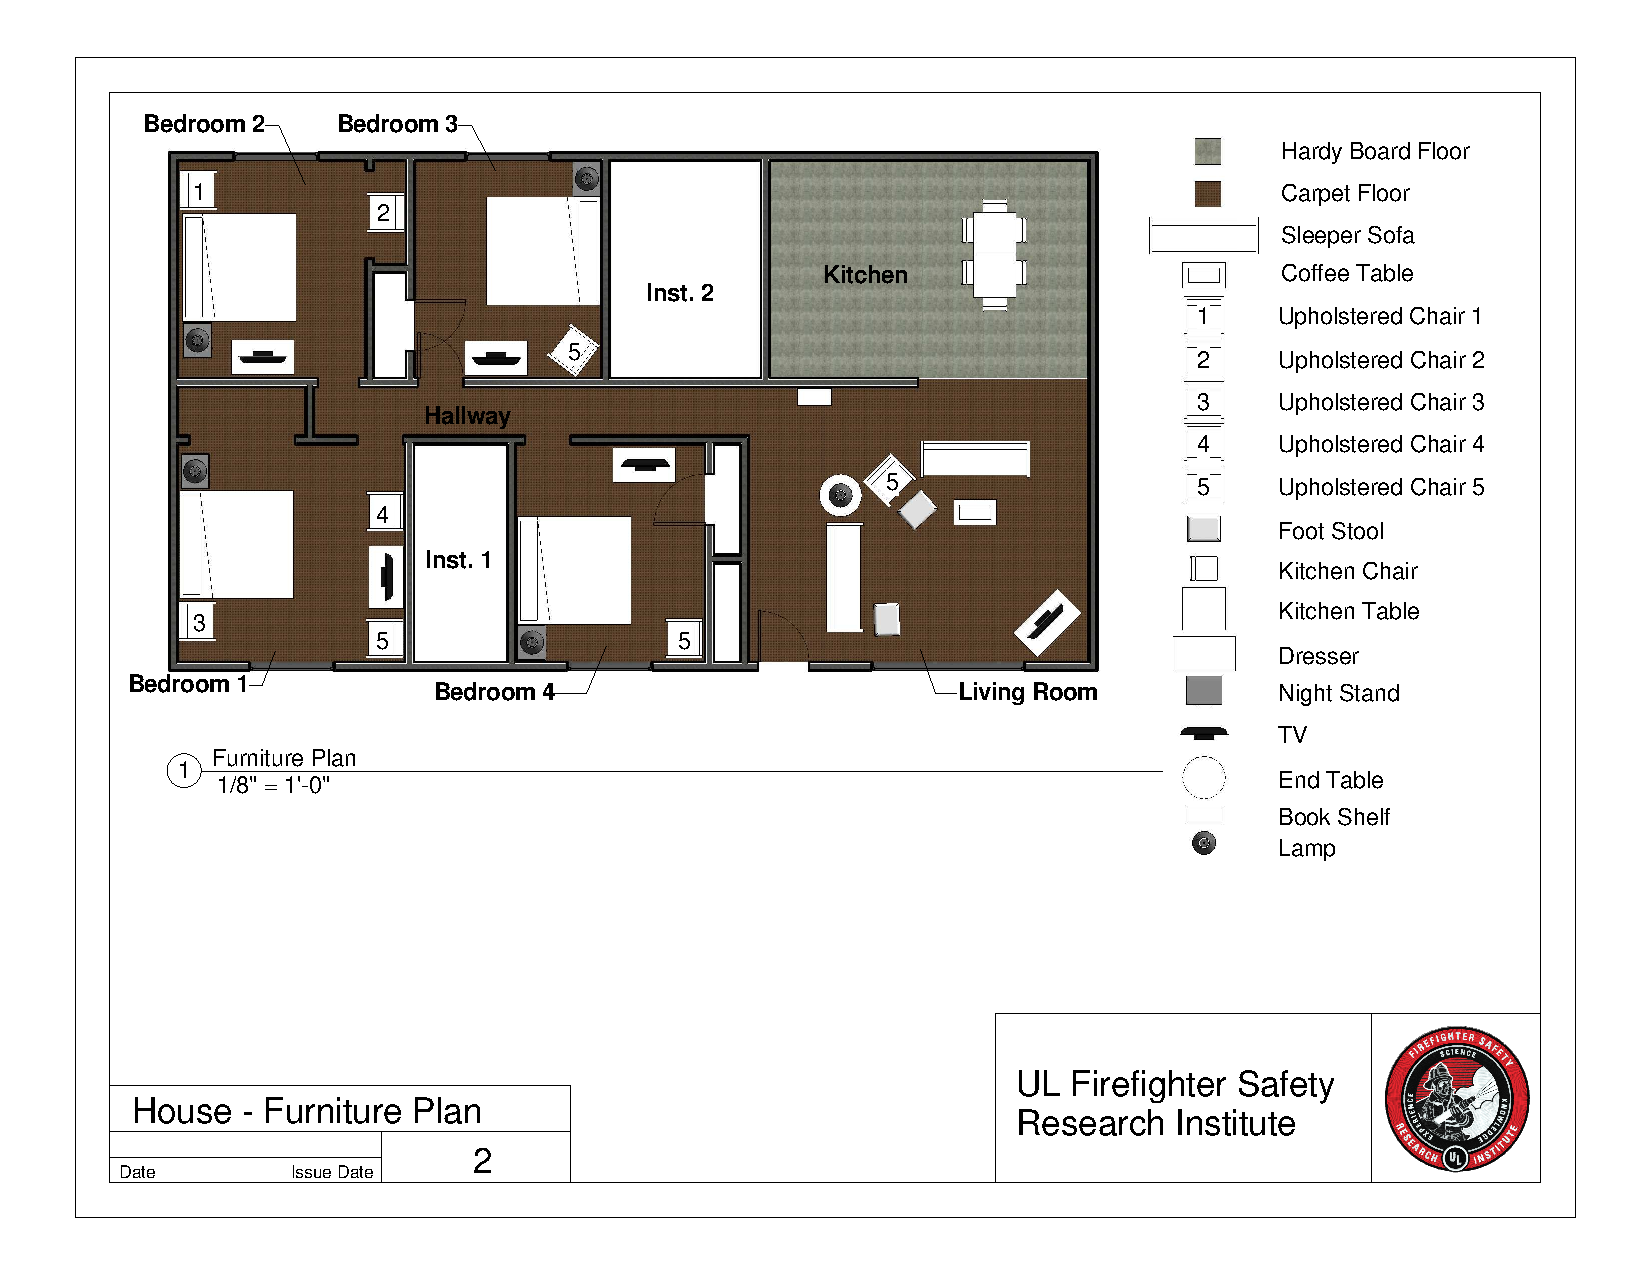
\includegraphics[width=\textheight]{../0_Images/Appendix_Figures/Furniture_Plan}
\caption[]{Test Fixture Furniture Plan}
\label{fig:appendix_furnitureplan}
\end{sidewaysfigure}

\begin{sidewaysfigure}
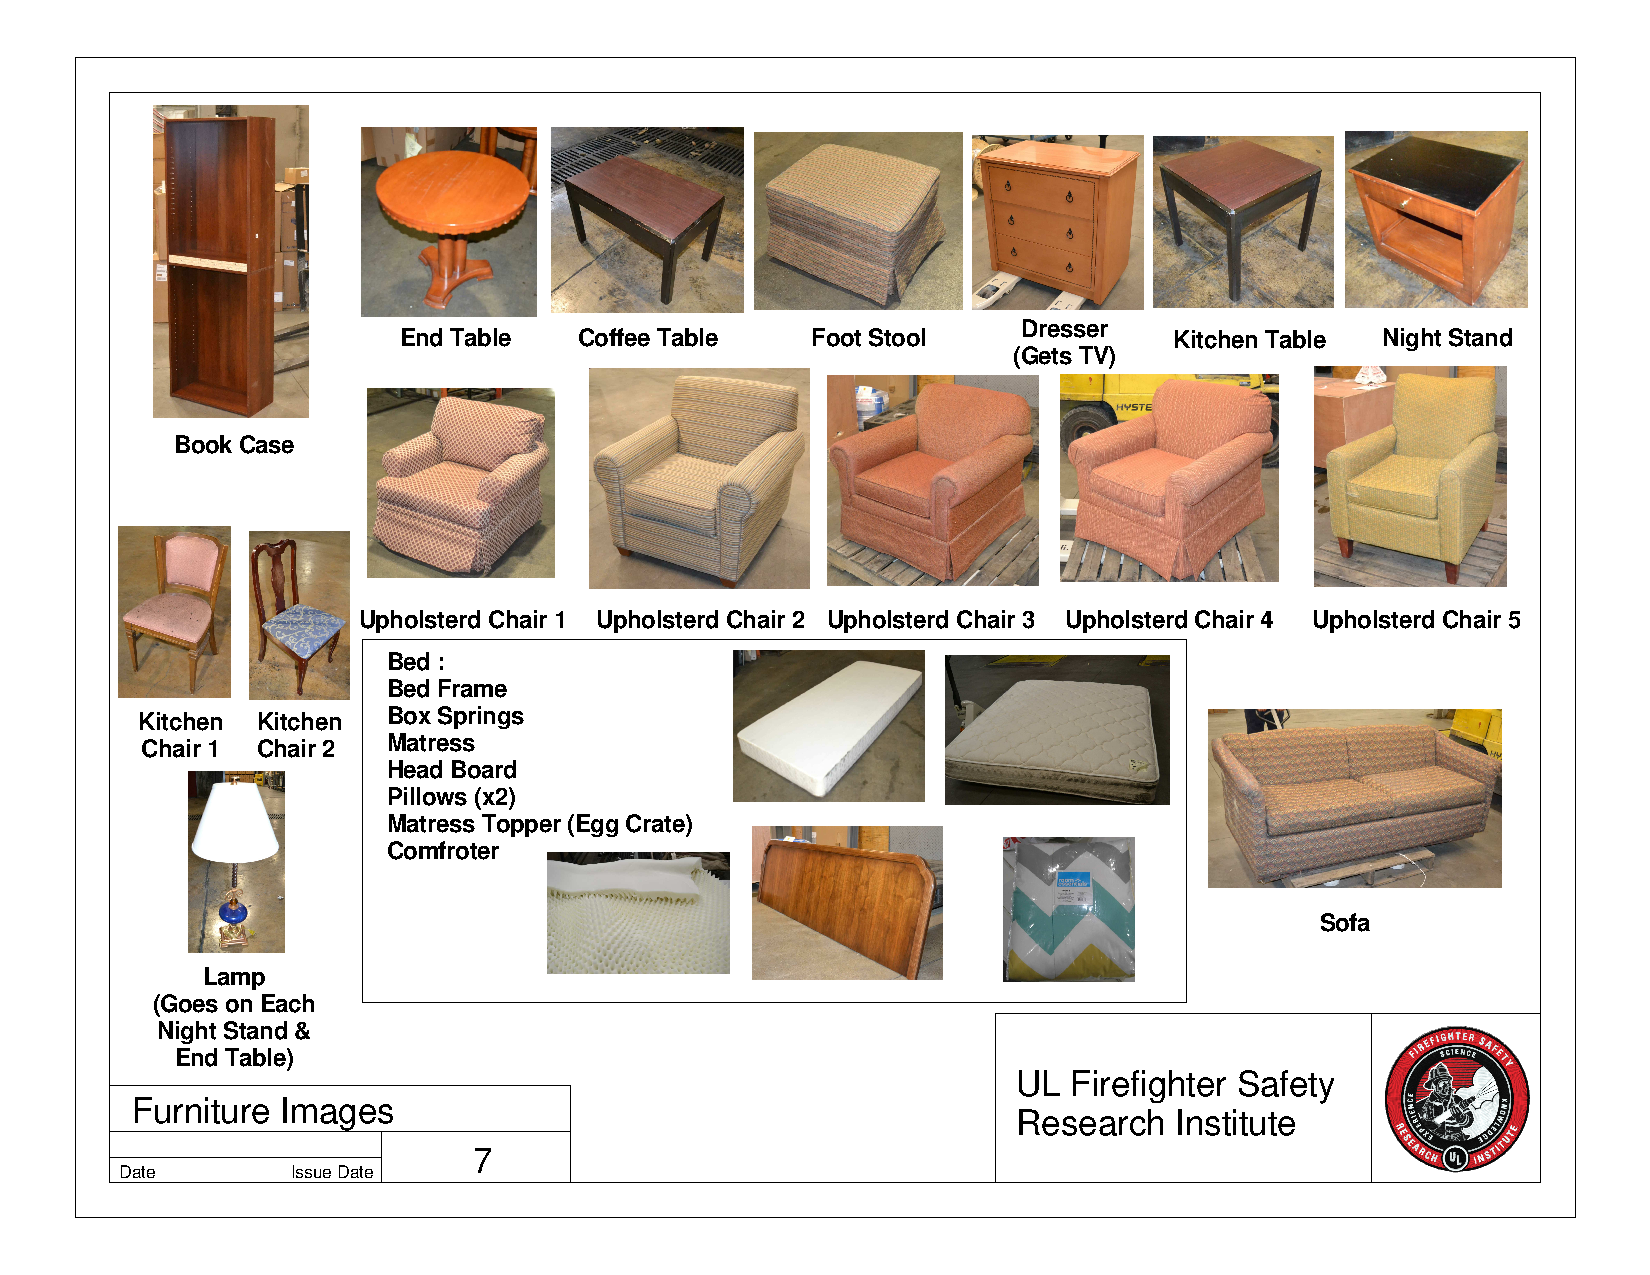
\includegraphics[width=\textheight]{../0_Images/Appendix_Figures/Furniture_Images}
\caption[]{Test Fixture Furniture Images}
\label{fig:appendix_furnitureimages}
\end{sidewaysfigure}

\begin{sidewaysfigure}
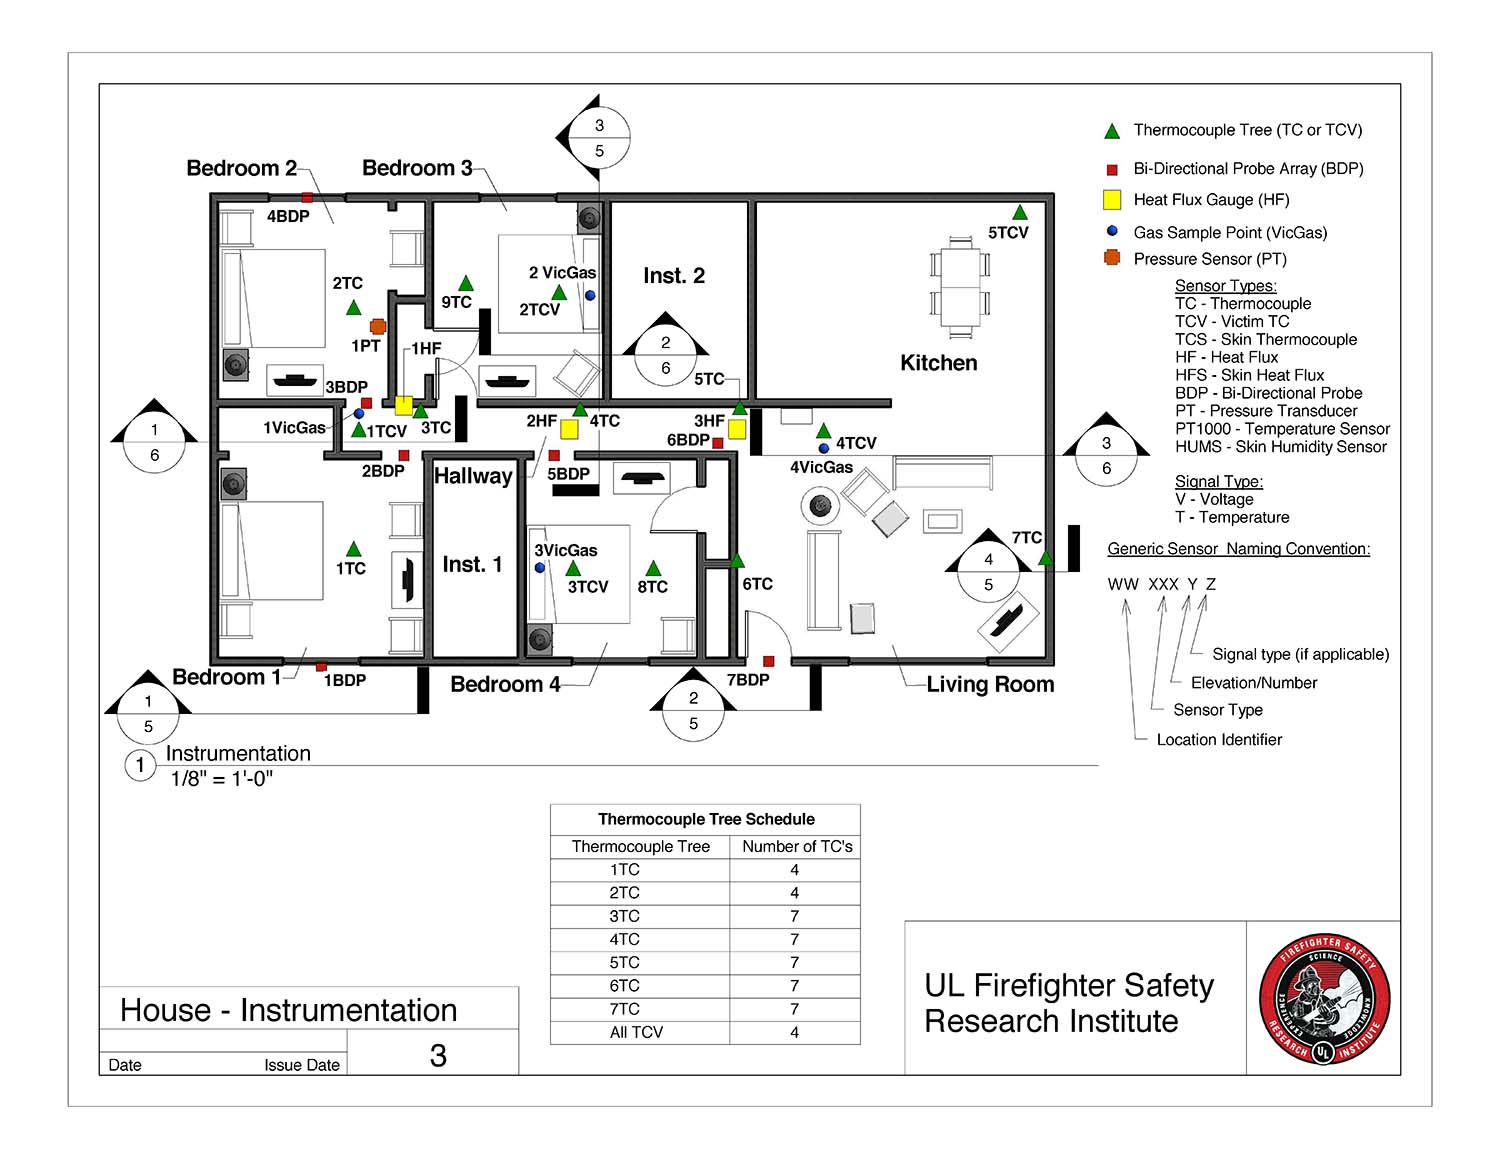
\includegraphics[width=\textheight]{../0_Images/Appendix_Figures/Instrument_Plan}
\caption[]{Instrumentation Plan}
\label{fig:appendix_instruments}
\end{sidewaysfigure}

\begin{sidewaysfigure}
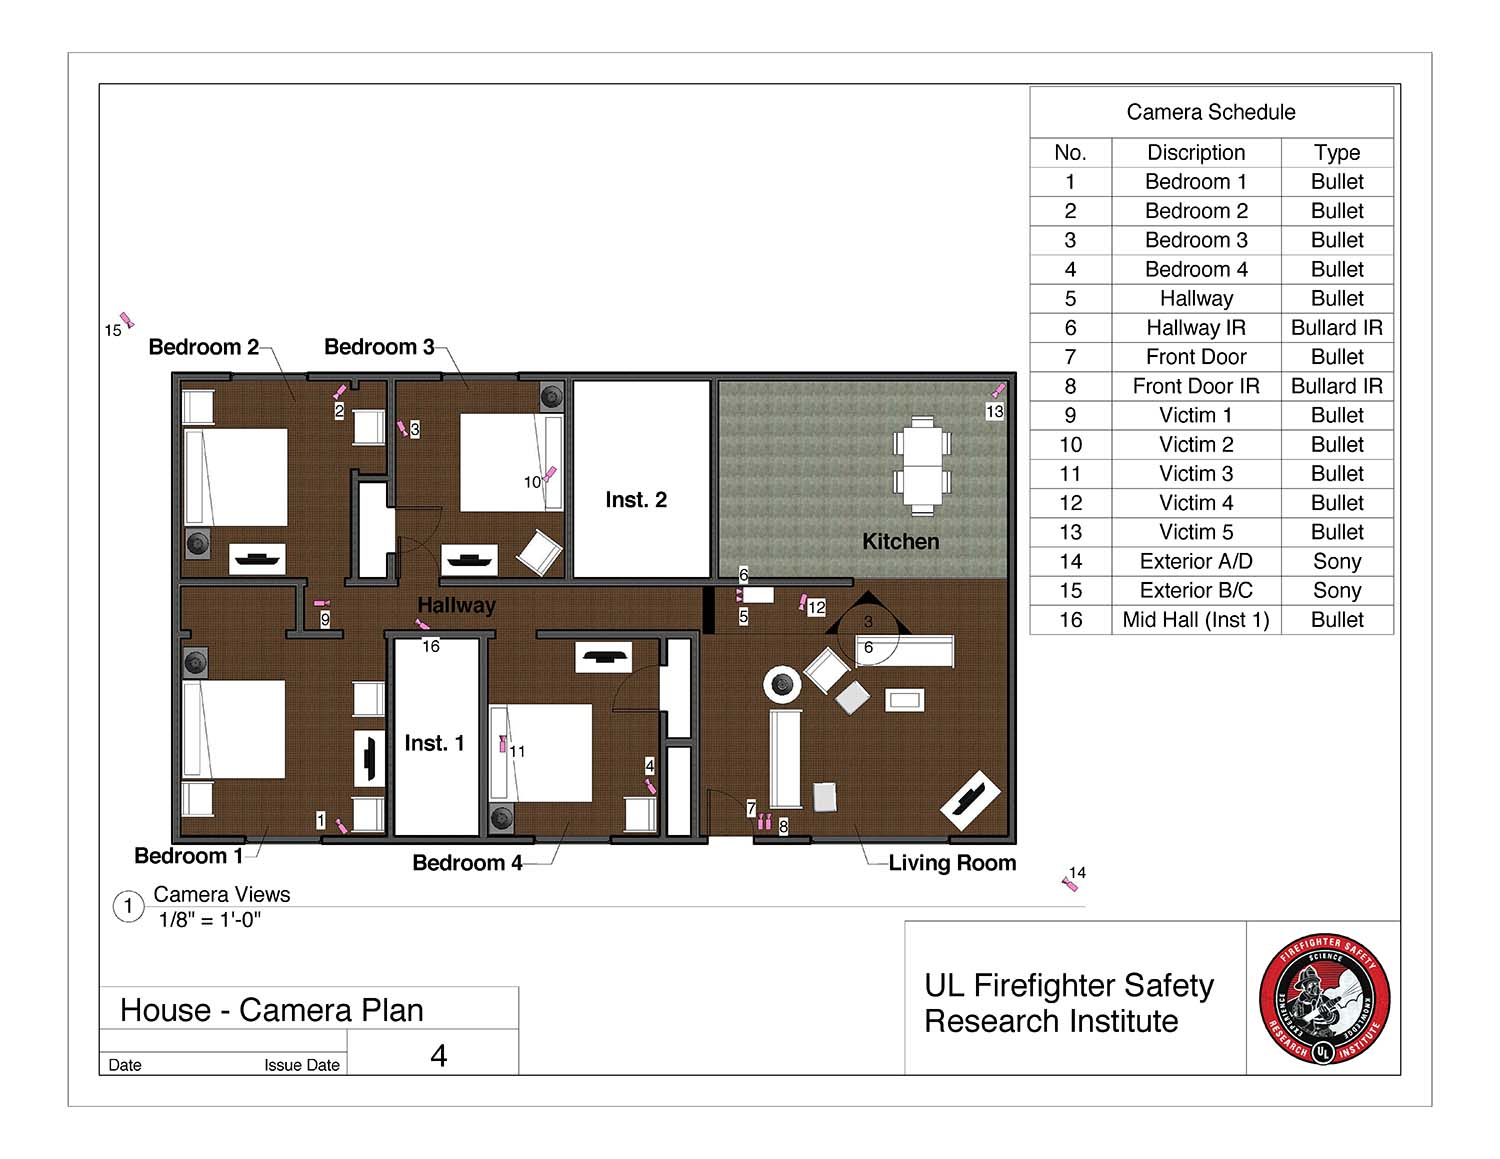
\includegraphics[width=\textheight]{../0_Images/Appendix_Figures/Camera_Plan}
\caption[]{Camera Plan}
\label{fig:appendix_cameras}
\end{sidewaysfigure}
